\documentclass[nojss]{jss}\usepackage[]{graphicx}\usepackage[]{color}
%% maxwidth is the original width if it is less than linewidth
%% otherwise use linewidth (to make sure the graphics do not exceed the margin)
\makeatletter
\def\maxwidth{ %
  \ifdim\Gin@nat@width>\linewidth
    \linewidth
  \else
    \Gin@nat@width
  \fi
}
\makeatother

\definecolor{fgcolor}{rgb}{0.345, 0.345, 0.345}
\newcommand{\hlnum}[1]{\textcolor[rgb]{0.686,0.059,0.569}{#1}}%
\newcommand{\hlstr}[1]{\textcolor[rgb]{0.192,0.494,0.8}{#1}}%
\newcommand{\hlcom}[1]{\textcolor[rgb]{0.678,0.584,0.686}{\textit{#1}}}%
\newcommand{\hlopt}[1]{\textcolor[rgb]{0,0,0}{#1}}%
\newcommand{\hlstd}[1]{\textcolor[rgb]{0.345,0.345,0.345}{#1}}%
\newcommand{\hlkwa}[1]{\textcolor[rgb]{0.161,0.373,0.58}{\textbf{#1}}}%
\newcommand{\hlkwb}[1]{\textcolor[rgb]{0.69,0.353,0.396}{#1}}%
\newcommand{\hlkwc}[1]{\textcolor[rgb]{0.333,0.667,0.333}{#1}}%
\newcommand{\hlkwd}[1]{\textcolor[rgb]{0.737,0.353,0.396}{\textbf{#1}}}%

\usepackage{framed}
\makeatletter
\newenvironment{kframe}{%
 \def\at@end@of@kframe{}%
 \ifinner\ifhmode%
  \def\at@end@of@kframe{\end{minipage}}%
  \begin{minipage}{\columnwidth}%
 \fi\fi%
 \def\FrameCommand##1{\hskip\@totalleftmargin \hskip-\fboxsep
 \colorbox{shadecolor}{##1}\hskip-\fboxsep
     % There is no \\@totalrightmargin, so:
     \hskip-\linewidth \hskip-\@totalleftmargin \hskip\columnwidth}%
 \MakeFramed {\advance\hsize-\width
   \@totalleftmargin\z@ \linewidth\hsize
   \@setminipage}}%
 {\par\unskip\endMakeFramed%
 \at@end@of@kframe}
\makeatother

\definecolor{shadecolor}{rgb}{.97, .97, .97}
\definecolor{messagecolor}{rgb}{0, 0, 0}
\definecolor{warningcolor}{rgb}{1, 0, 1}
\definecolor{errorcolor}{rgb}{1, 0, 0}
\newenvironment{knitrout}{}{} % an empty environment to be redefined in TeX

\usepackage{alltt}

%%%%%%%%%%%%%%%%%%%%%%%%%%%%%%
%% declarations for jss.cls %%
%%%%%%%%%%%%%%%%%%%%%%%%%%%%%%
%\VignetteEngine{knitr::knitr}
%\VignetteIndexEntry{hviPlotR}
%\VignetteIndexEntry{Generating plot.sas style figures in R}
%\VignetteKeywords{publication graphics, powerpoint, ggplot2, plot.sas}
%\VignetteDepends{ggplot2}
%\VignettePackage{hviPlotR} 

\usepackage{float}
\usepackage{listings}
\usepackage{color}

\definecolor{mygreen}{rgb}{0,0.6,0}
\definecolor{mygray}{rgb}{0.95,0.95,0.95}
\definecolor{mymauve}{rgb}{0.58,0,0.82}
\lstset{
backgroundcolor=\color{mygray},   % choose the background color; you must add \usepackage{color} or \usepackage{xcolor}
basicstyle=\ttfamily\footnotesize,
breakatwhitespace=false,         % sets if automatic breaks should only happen at whitespace
breaklines=true,                 % sets automatic line breaking
captionpos=b,                    % sets the caption-position to bottom
commentstyle=\color{mygreen},    % comment style
%deletekeywords={...},            % if you want to delete keywords from the given language
escapeinside={\%*}{*)},          % if you want to add LaTeX within your code
extendedchars=true,              % lets you use non-ASCII characters; for 8-bits encodings only, does not work with UTF-8
%frame=single,                    % adds a frame around the code
keepspaces=true,                 % keeps spaces in text, useful for keeping indentation of code (possibly needs columns=flexible)
keywordstyle=\color{blue},       % keyword style
language={SAS},                  % the language of the code
morekeywords={*,...},            % if you want to add more keywords to the set
numbers=none,                    % where to put the line-numbers; possible values are (none, left, right)
%numbersep=5pt,                   % how far the line-numbers are from the code
%numberstyle=\tiny\color{mygray}, % the style that is used for the line-numbers
%rulecolor=\color{black},         % if not set, the frame-color may be changed on line-breaks within not-black text (e.g. comments (green here))
showspaces=false,                % show spaces everywhere adding particular underscores; it overrides 'showstringspaces'
showstringspaces=false,          % underline spaces within strings only
showtabs=false,                  % show tabs within strings adding particular underscores
%stepnumber=2,                    % the step between two line-numbers. If it's 1, each line will be numbered
stringstyle=\color{mymauve},     % string literal style
tabsize=2,                       % sets default tabsize to 2 spaces
title=\lstname                   % show the filename of files included with \lstinputlisting; also try caption instead of title
}

%% almost as usual
\author{John Ehrlinger\\Quantitative Health Sciences\\Lerner Research Institute\\Cleveland Clinic} %\And \\Plus Affiliation}
\title{The {\pkg{hviPlotR}} package: Generating \code{plot.sas} style figures in \proglang{R}}

%% for pretty printing and a nice hypersummary also set:
\Plainauthor{John Ehrlinger} %% comma-separated
\Plaintitle{hviPlotR: Generating plot.sas style figures in R} %% without formatting
\Shorttitle{hviPlotR: Generating plot.sas style figures}

%% an abstract and keywords
\Abstract{ 
We introduce the \proglang{R} package \pkg{hviPlotR}, a set of tools for creating publication quality graphics in \proglang{R}. The \pkg{hviPlotR} package is designed to replace the \code{plot.sas} macro we currently use in \proglang{SAS}. The package includes both \proglang{R} recipes for generating our standard graphics using \pkg{ggplot2} commands and a set of themes designed to format those figures for both manuscript and \code{PowerPoint} targets. 

The goal of this package vignette is to introduce the \pkg{hviPlotR} methodology, as well as to document the best practices of creating our publication quality graphics for both manuscripts and power point presentations.

This document is included with the \pkg{hviPlotR} package as a package vignette, installed into \proglang{R} when the package is installed, and view able using the \code{vignette("hviPlotR")} command.
}
\Keywords{publication graphics, powerpoint, ggplot2, plot.sas}
\Plainkeywords{publication graphics, powerpoint, ggplot2, plot.sas}
%% at least one keyword must be supplied

%% publication information
%% NOTE: Typically, this can be left commented and will be filled out by the technical editor
%% \Volume{13}
%% \Issue{9}
%% \Month{September}
%% \Year{2004}
%% \Submitdate{2004-09-29}
%% \Acceptdate{2004-09-29}

%% The address of (at least) one author should be given
%% in the following format:
\Address{
John Ehrlinger\\
Quantitative Health Sciences\\
Lerner Research Institute\\
Cleveland Clinic\\
9500 Euclid Ave\\
Cleveland, Ohio 44195\\
%  Telephone: +41/0/44634-4643 \\
%  Fax: +41/0/44634-4386 \\
E-mail: \email{john.ehrlinger@gmail.com}\\
URL: \url{http://www.lerner.ccf.org/qhs/people/ehrlinj/}\\
URL: \url{https://github.com/ehrlinger/hviPlotR}
}

%% It is also possible to add a telephone and fax number
%% before the e-mail in the following format:
%% Telephone: +43/1/31336-5053
%% Fax: +43/1/31336-734

%% for those who use Sweave please include the following line (with % symbols):
%% need no \usepackage{Sweave.sty}

%% end of declarations %%%%%%%%%%%%%%%%%%%%%%%%%%%%%%%%%%%%%%%%%%%%%%%



\IfFileExists{upquote.sty}{\usepackage{upquote}}{}
\begin{document}

%% include your article here, just as usual
%% Note that you should use the \pkg{}, \proglang{} and \code{} commands.

\begin{knitrout}\footnotesize
\definecolor{shadecolor}{rgb}{0.969, 0.969, 0.969}\color{fgcolor}\begin{figure}[htpb]


{\centering 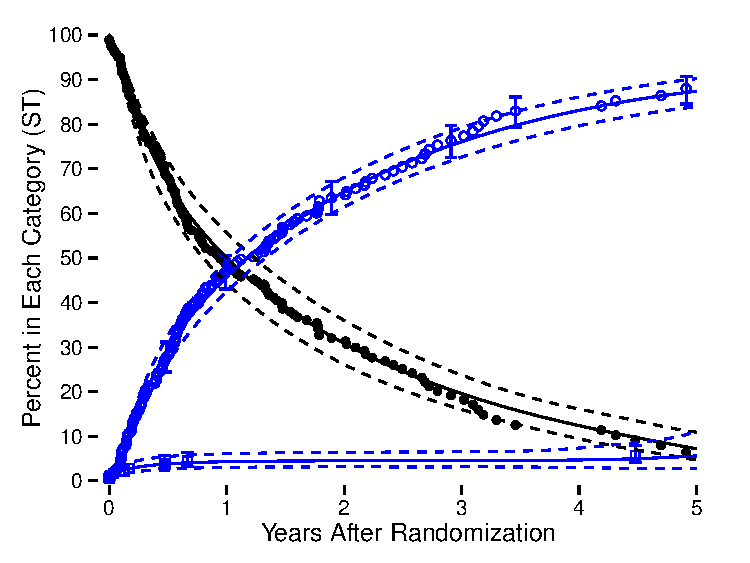
\includegraphics[width=\maxwidth]{figure/beamer-introFigure} 

}

\caption[Demonstration figure]{Demonstration figure\label{F:introFigure}}
\end{figure}


\end{knitrout}

% -----------------------------------------------------
\section{About this document}
% -----------------------------------------------------
This document is an introduction to the \proglang{R} package \pkg{hviPlotR}, a set of tools for creating publication quality graphics in \proglang{R}. The package and this document describe the process of creating graphics in \proglang{R} that conform to the standards of the clinical investigations statistics group within The Heart \& Vascular Institute at the Cleveland Clinic. These graphics are analogous to those generated with the \code{plot.sas} macro in \proglang{SAS}.

This document is the package vignette for the \pkg{hviPlotR} package, and as such is the primary documentation for the package. The latest version of the document can be obtained with the 
\begin{CodeChunk}
\begin{CodeInput}
R> vignette("hviPlotR", package = "hviPlotR")
\end{CodeInput}
\end{CodeChunk}

The goal is to update this document as the package is updated to include all relevant changes for publication. 

% -----------------------------------------------------
\section{Introduction}
% -----------------------------------------------------
For many years, the mainstay for generating graphics for manuscripts and presentations in the statistics group in HVI has been the \code{plot.sas} macro using \proglang{SAS}. However, recently, we have had issues migrating this macro to newer versions of \proglang{SAS} ($> 8.0$) and MicroSoft Office products ($> 2003$). 

In an effort to alleviate the versifying problems, and to standardize the generation of figures within \proglang{R}, we have developed the \pkg{hviPlotR} \proglang{R} package. The goal of the package, and this document, is simplify the creation of publication quality graphics in  \proglang{R}. We are specifically encoding the best practices of the HVI Clinical Investigations formatting, so that our statisticians will be able to simply create graphics for publication with a minimal amount of effort.

The \pkg{hviPlotR} package also implements best practices for \proglang{R} graphics by leveraging the \pkg{ggplot2} package~\citep{Wickham:2009}. The \pkg{ggplot2} package is an implementation of the Grammar of Graphics~\citep{Wilkinson:2005}, which is a formalization of graphical concepts, and the building of graphical objects from a sequence of independent components. These components can be combined in many different ways.

The \code{plot.sas} macro is also an implementation of a graphics grammar. The grammar is derived from the ZETA pen plotters, which used GML (Graphics Machine Language) to control between 4 and and 8 colored pens for generating color line and point figures. Because both systems use a graphics language it is straight forward to translate commands between the two methods. 

This document outlines how to generate figures using the \pkg{ggplot2} and \pkg{hviPlotR} packages. Our approach is to demonstrate the \proglang{R} commands to generate the same elements created with \code{plot.sas} commands. Section~\ref{S:plot.sas} gives an overview of the methodology of the \code{plot.sas} macro and Section~\ref{S:ggplot2tuple} details how to create line and point plots with \pkg{ggplot2}. A key part of \pkg{hviPlotR} package is custom themes for figures. Once you have created your figure, Section~\ref{S:themes} details how to get the formatting correct for manuscripts or presentations. Section~\ref{S:saving} describes functions for saving the figures to simplify the import into publication documents.

% -----------------------------------------------------
\section[The plot.sas macro]{The \code{plot.sas} macro}\label{S:plot.sas}
% -----------------------------------------------------

To demonstrate the process, we first look at some example code using the \code{plot.sas} macro. This code is intended to generate a figure for manuscript publication and was modified to generate Figure~\ref{F:introFigure}.
\begin{lstlisting}[float,floatplacement=!htpb, caption={plot.sas commands: Figure setup.},label={plot.sas:figureSetup}]
%let STUDY=/studies/cardiac/valves/aortic/replacement/partner_publication_office/partner1b/mortality_5y
*****************************************************************************;
* Bring in PostScript plot macro                                             ;
filename plt "!MACROS/plot.sas"; %inc plt;
filename gsasfile pipe 'lp';
*____________________________________________________________________________;
*                                                                            ;
*                       P O S T S C R I P T   P L O T S
*____________________________________________________________________________;
* Multiple decrement, nonparametric and parametric                           ;
filename gsasfile "&STUDY/graphs/ce.states.ST.ps";

*____________________________________________________________________________;
* Create the figure here   !                                                 ;
*____________________________________________________________________________;
%plot(goptions gsfmode=replace, device=pscolor, gaccess=gsasfile end;
      id l="&STUDY/graphs/ce.states.ST.sas percent", end;
     labelx l="Years After Randomization", end;
     axisx order=(0 to 5 by 1), minor=none, end;
     labely l="Percent in Each Category (ST)", end;
     axisy order=(0 to 100 by 10), minor=none, end;
\end{lstlisting}

Note the first line of the code block in Listing~\ref{plot.sas:figureSetup} indicates the path to the file location. The \code{filename} statments bring in the \code{plot.sas} macro, indicate how to print, and where to save the graphics file. The \code{plot.sas} macro call starts with the \code{\%plot} command. The first line sets global graphic values, including the file where the figure will be saved (see Section~\ref{S:saving}). Each \code{plot.sas} command is terminated with the \code{end;} statement. We'll look at each command type individually.

The \code{id l=} command sets the footnote text used for manuscript figures to identify where the figure is saved (see Section~\ref{S:saving}). The \code{labelx} and \code{labely} commands set the axis label text (Section~\ref{S:labels}) and the \code{axisx} and \code{axisy} set the scales for each axis locating text and tics (Section~\ref{S:scales}).

\begin{lstlisting}[float,floatplacement=!htpb, caption={plot.sas commands: points and errorbar tuple statements.}\label{plot.sas:pointTuple}]
/******NON-PARAMETRIC: SYMBOLS AND CONFIDENCE BARS *******/
tuple set=green, symbol=dot, symbsize=1/2, linepe=0, linecl=0,
     ebarsize=3/4, ebar=1,
     x=iv_state, y=sginit, cll=stlinit, clu=stuinit, color=black, 
     end;
tuple set=green, symbol=circle, symbsize=1/2, linepe=0, linecl=0,
     ebarsize=3/4, ebar=1,
     x=iv_state, y=sgdead1, cll=stldead1, clu=studead1, color=blue, 
     end;
tuple set=green, symbol=square, symbsize=1/2, linepe=0, linecl=0,
     ebarsize=3/4, ebar=1,
     x=iv_state, y=sgstrk1, cll=stlstrk1, clu=stustrk1, color=blue, 
     end;
\end{lstlisting}
The \code{tuple} command builds up graphics objects within the figure plot window. The first set of tuple commands builds up a set of three elements containing both points (Section~\ref{S:points}) and errorbars (Section~\ref{S:errorbars}). Each \code{tuple} statement operates on a dataset indicated by the \code{set} command. 

Symbols shapes and sizes are specified with the \code{symbol} and \code{symbsize} commands (Section~\ref{S:shapes}).

The second set of \code{tuple} statements build up a set of three elements containing lines and confidence intervals (Section~\ref{S:lines}).
\begin{lstlisting}[float,floatplacement=!htpb, caption={plot.sas commands: lines tuple statements.}, label={plot.sas:linesTuple}]
/**********PARAMETRIC : SOLID LINES AND CONFIDENCE INTERVALS**********/      
tuple set=all, x=years, y=noinit, cll=clinit, clu=cuinit,
     width=0.5,color=black, 
     end;

tuple set=all, x=years, y=nodeath, cll=cldeath, clu=cudeath,
     width=0.5,color=blue, 
     end;

tuple set=all, x=years, y=nostrk, cll=clstrk, clu=custrk,
     linecl=2, width=0.5,color=blue, 
     end;
);
run;
*****************************************************************************;
\end{lstlisting}

The \code{plot.sas} macro code is closed by the ending \code{);} characters, and \proglang{SAS} is instructed to \code{run;} the code. Running combines building the figure by combining elements from \code{label}, \code{axis} and \code{tuple} statements and saving it into the file specified by the \code{gsasfile} variable. The resulting figure is shown in Figure~\ref{F:sasManuscript}.

\begin{figure}[!htpb]
\centering
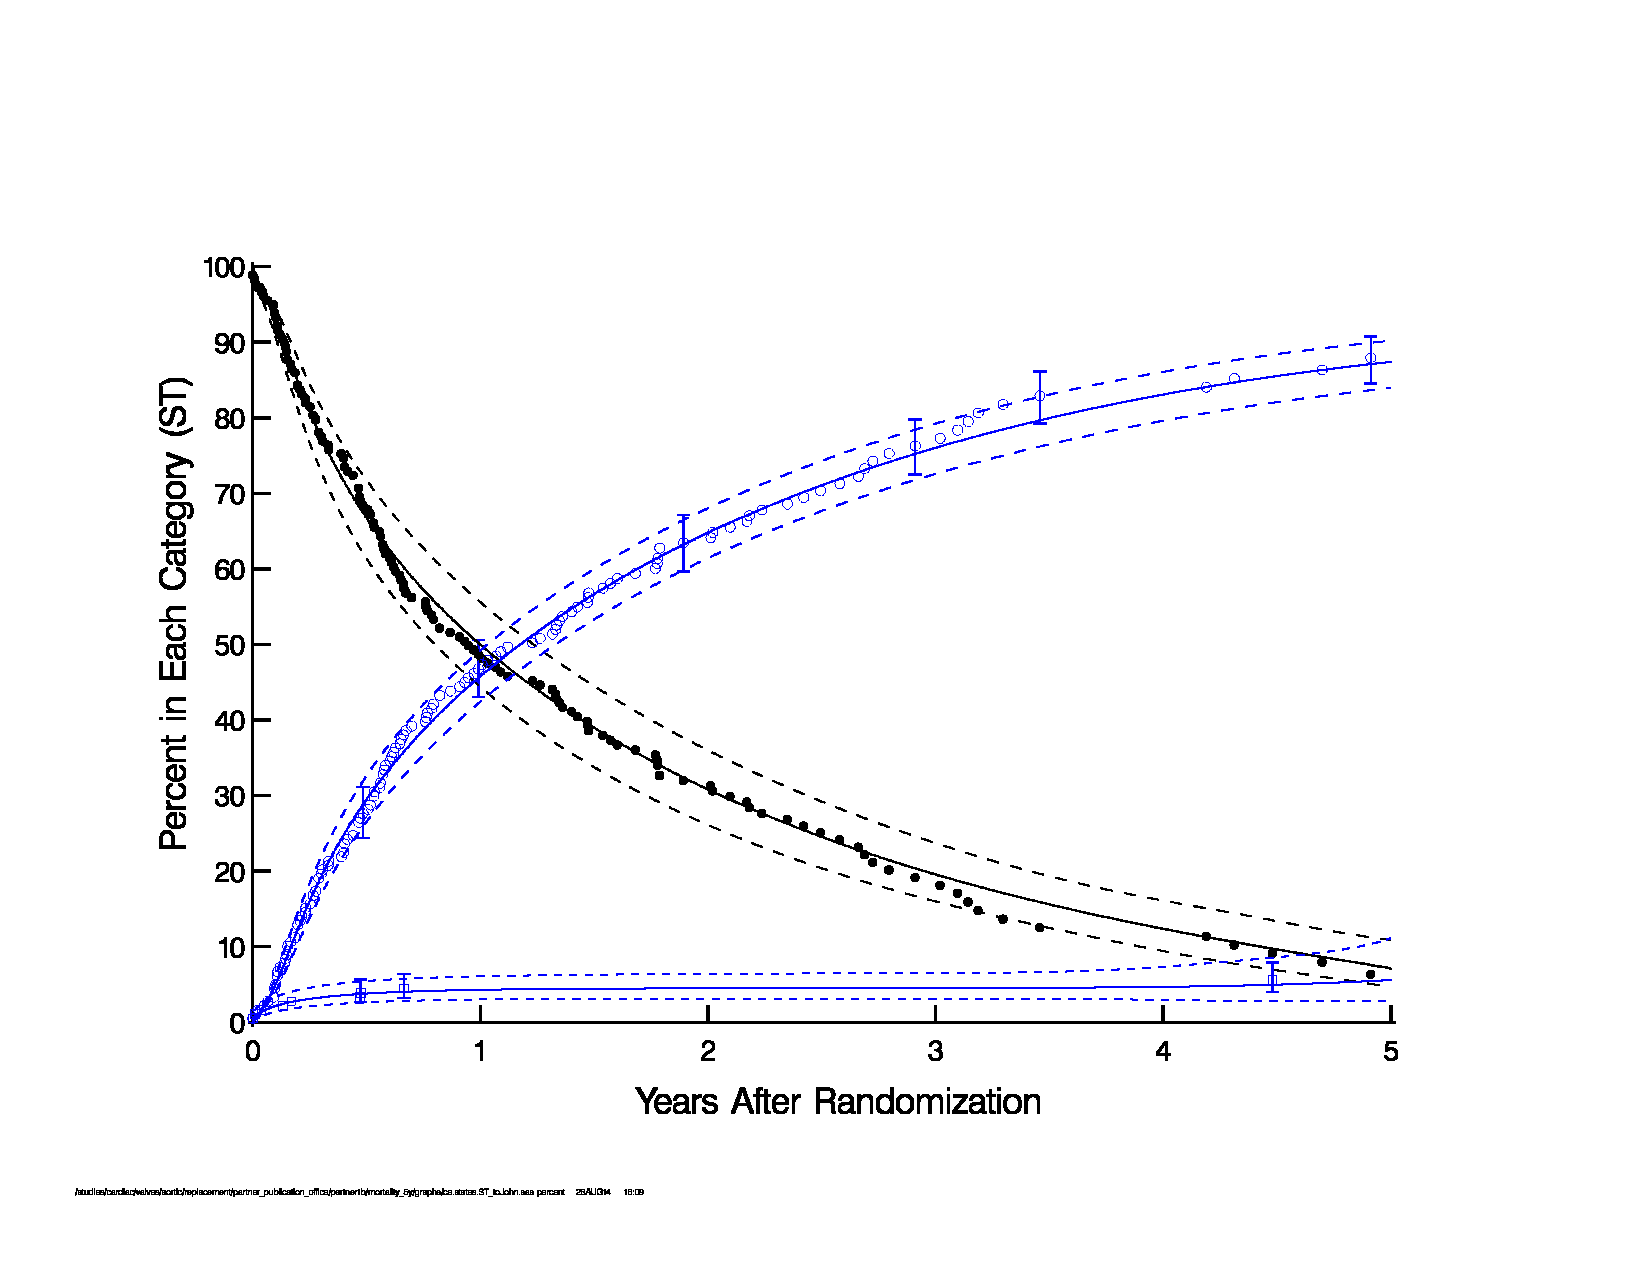
\includegraphics[width=0.8\textwidth]{../inst/ceStatesST.pdf}
\caption{Manuscript figure (SAS version)}
\label{F:sasManuscript}
\end{figure}

Note that much of the figure formatting is mixed within the \code{tuple} statements using \code{width}, \code{color}, \code{linepe} and \code{linecl} commands. In the \code{plot.sas} macro, omitting these commands will generate a figure with the default values specified within the \code{device} theme (Section~\ref{S:themes}).


A similar set of \code{plot.sas} commands is used to create presentation graphics.
\begin{lstlisting}[float,floatplacement=!htpb, caption={plot.sas commands: CGM instructions.}, label={plot.sas:cgm}]
*____________________________________________________________________________;
*                                                                            ;
*       C G M   F I L E S   F O R   P O W E R P O I N T   S L I D E S
*____________________________________________________________________________;
* Competing risks, parametric only                                           ;
filename gsasfile "&STUDY/graphs/ce.states.ST.cgm";
%plot(goptions gsfmode=replace, device=cgmmppa, ftext=hwcgm001, end;
     axisx order=(0 to 5 by 1), minor=none, value=(height=2.4), end;
     axisy order=(0 to 100 by 20), minor=none, value=(height=2.4), 
     value=(height=2.4 j=r ' ' '20' '40' '60' '80' '100'), end;
     tuple set=all, x=years, y=noinit, width=3, color=gray, end;
     tuple set=all, x=years, y=nostrk, width=3, color=red, end;
     tuple set=all, x=years, y=nodeath, width=3, color=blue, end;
);
run;  
\end{lstlisting}
%\caption{SAS Code for powerpoint figure.\label{C:powerpoint}}
Differences include the target \code{device} and \code{ftext} as well as some handling of figure labels with \code{value} instead of \code{label} commands. We also have rules for what to and not to include in presentation graphics (Section~\ref{S:rules}).

\begin{figure}[!htpb]
\centering
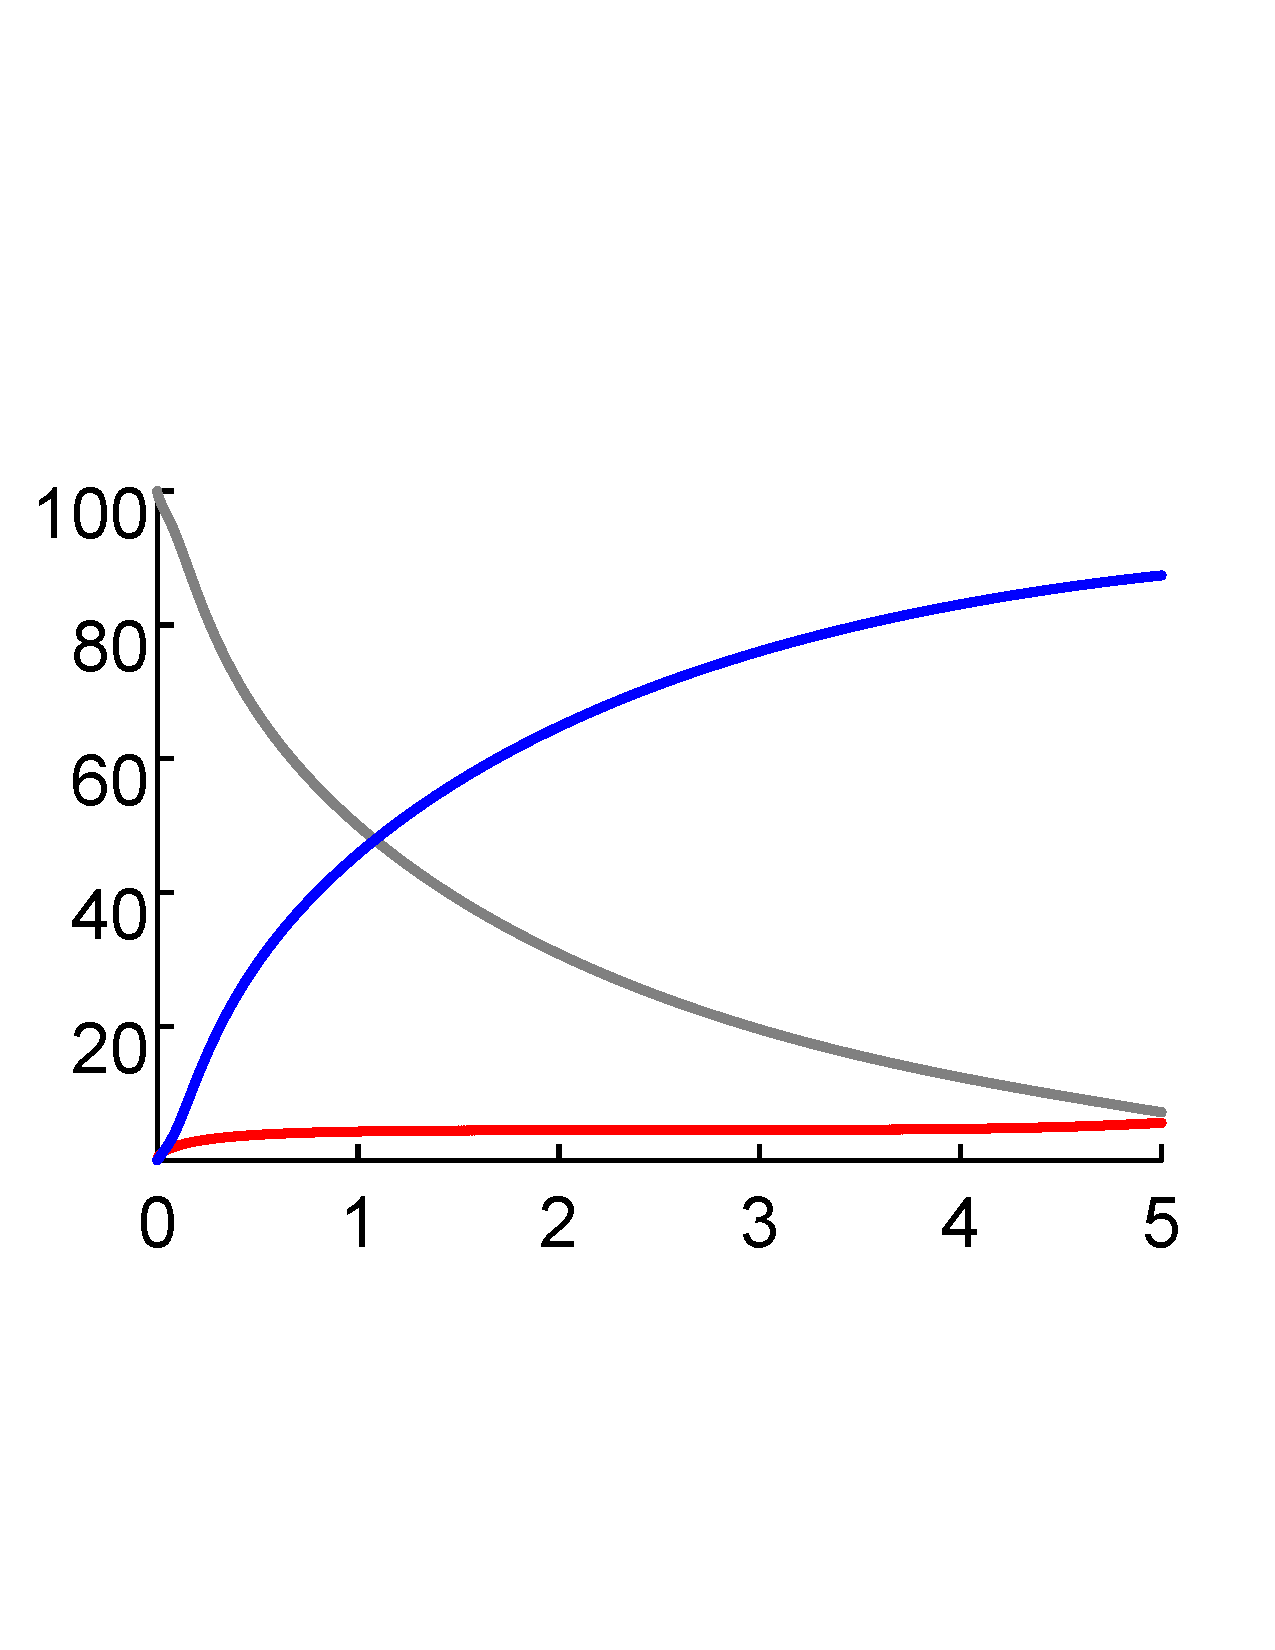
\includegraphics[width=0.8\textwidth]{../inst/ceStatesST_ppt.pdf}
\caption{PowerPoint figure (SAS version)}
\label{F:sasPowerPoint}
\end{figure}

% -----------------------------------------------------
\section[Generating ggplot2 graphics]{Generating \pkg{ggplot2} graphics}\label{S:ggplot2tuple}
% -----------------------------------------------------

In order to create figures similar to the \code{plot.sas} macro, using \proglang{R}, we will make extensive use of the \pkg{ggplot2} package. This will require translating from the graphics language of \code{plot.sas} to the graphics language of \pkg{ggplot2}. 

For the remainder of this document, \proglang{R} code will be highlighted in grey boxes, as shown below. We will refer to these blocks as \emph{code chunks}. You can run each code chunk individuallym, using copy/paste into an interactive \proglang{R} session, or a stand alone \proglang{R} script.

This tutorial requires the \pkg{hviPlotR} package for data and themes we will be discussing. You can load it with the following commands:
\begin{knitrout}\footnotesize
\definecolor{shadecolor}{rgb}{0.969, 0.969, 0.969}\color{fgcolor}\begin{kframe}
\begin{alltt}
\hlcom{# Install the latest hviPlotR package.}
\hlcom{#}
\hlcom{# The devtools package is installed on all our }
\hlcom{# jjnb-gen servers as well as other R instances.}
\hlkwd{library}\hlstd{(devtools)}

\hlcom{# To get the latest version.}
\hlkwd{install_github}\hlstd{(}\hlstr{"ehrlinger/hviPlotR"}\hlstd{)}
\end{alltt}
\end{kframe}
\end{knitrout}


\subsection{Initialize the figure}\label{S:initial}
Refering back to the \proglang{SAS} code chunks in Section~\ref{S:plot.sas}, the first section of the code sets the current working directory, and does some house keeping, including loading the \code{plot.sas} macro. Similarly, to get started in \proglang{R}, we first load the required libraries: \pkg{ggplot2} for graphics, and \pkg{hviPlotR} for themes. The following code chunk also sets the initial default theme to a generic black and white format, and brings in a pair of example datasets. 
\begin{knitrout}\footnotesize
\definecolor{shadecolor}{rgb}{0.969, 0.969, 0.969}\color{fgcolor}\begin{kframe}
\begin{alltt}
\hlcom{# load required libraries}
\hlkwd{library}\hlstd{(ggplot2)}   \hlcom{# Plotting environment}
\hlkwd{library}\hlstd{(hviPlotR)}  \hlcom{# CCF HVI plotting functionality }

\hlkwd{theme_set}\hlstd{(}\hlkwd{theme_bw}\hlstd{())} \hlcom{# A reasonable default plotting theme}

\hlcom{# Load the example datasets }
\hlkwd{data}\hlstd{(parametric,} \hlkwc{package}\hlstd{=}\hlstr{"hviPlotR"}\hlstd{)}
\hlkwd{data}\hlstd{(nonparametric,} \hlkwc{package}\hlstd{=}\hlstr{"hviPlotR"}\hlstd{)}
\end{alltt}
\end{kframe}
\end{knitrout}


One advantage of \pkg{ggplot2} is that figures can be built up in successive statements. This tutorial will make extensive use of this to demonstrate the process. Starting in this code chunk, we will save the intermediate objects in the \code{ccf_plot} variable. Here we simply create an empty \pkg{ggplot2} figure that we will be adding to as we work through the commands in the \code{plot.sas} macro. Note that we include the  \code{\%plot()} command in the comment above the equivalent \pkg{ggplot2} command.
\begin{knitrout}\footnotesize
\definecolor{shadecolor}{rgb}{0.969, 0.969, 0.969}\color{fgcolor}\begin{kframe}
\begin{alltt}
\hlcom{## To reproduce the plot.sas function, line by line.}
\hlcom{###-------------}
\hlcom{## There are SAS options we will not use here.}
\hlcom{#}
\hlcom{#  %plot(goptions gsfmode=replace, device=pscolor, gaccess=gsasfile end;}
\hlstd{ccf_plot} \hlkwb{<-} \hlkwd{ggplot}\hlstd{()}
\end{alltt}
\end{kframe}
\end{knitrout}

\subsection{Labels}\label{S:labels}
The next section of the \proglang{SAS} code in Section~\ref{S:plot.sas} sets the x and y axis titles, as well as the location of the majoe axis tick marks. We will splot this up for our \proglang{R} code.  \pkg{ggplot2} uses a \code{labs} function to set the axis labels. 
\begin{knitrout}\footnotesize
\definecolor{shadecolor}{rgb}{0.969, 0.969, 0.969}\color{fgcolor}\begin{kframe}
\begin{alltt}
\hlcom{###-------------}
\hlcom{## Labels are a single command, scales control the axis}
\hlcom{#}
\hlcom{#    labelx l="Years After Randomization", end;}
\hlcom{#    labely l="Percent in Each Category (ST)", end;}
\hlstd{ccf_plot} \hlkwb{<-} \hlstd{ccf_plot} \hlopt{+}
  \hlkwd{labs}\hlstd{(}\hlkwc{x}\hlstd{=}\hlstr{"Years After Randomization"}\hlstd{,}
       \hlkwc{y}\hlstd{=}\hlstr{"Percent in Each Category (ST)"}\hlstd{)}
\end{alltt}
\end{kframe}
\end{knitrout}

The \code{labs} function can also be used to set the plot \code{title} and legend titles. We will not cover that functionality here, details are available in~\cite{Wickham:2009} or through the Internet.

\subsection{Scales}\label{S:scales}
Axis ticks are controled with the \code{scale} functions. \pkg{ggplot2} has many different \code{scale} functions. These functions will work on one axis at a time, so for a typical continous axis, we refer to the \code{scale_x_continuous} or \code{scale_y_continuous} functions. Major axis are controlled using the \code{breaks} argument. This code uses a sequence of numbers to set the location of major tick marks (\code{seq(0,5,1)}). One mark for every year starting at 0, and ending at 5. Minor tick marks are automatically generated, but can also be specified using a \code{minor_breaks=} argument. You could also specifiy the breaks using a vector of values (\code{c(0,1,2,3,4,5)}), as well as relabel the ticks manually using a \code{labels=} argument.

Note that the \code{scale_} functions do not restrict the figure viewport at all. They are simply used to setup the axis tick marks. You can specify that the y-axis ticks are only from 0 to 50, and the figure would have a blank from 50 to the limits of the data. We discuss controlling the figure viewport in Section~\ref{S:globals}.

\begin{knitrout}\footnotesize
\definecolor{shadecolor}{rgb}{0.969, 0.969, 0.969}\color{fgcolor}\begin{kframe}
\begin{alltt}
\hlcom{###-------------}
\hlcom{## Labels are a single command, scales control the axis}
\hlcom{#}
\hlcom{#      axisx order=(0 to 5 by 1), minor=none, end;}
\hlcom{#      axisy order=(0 to 100 by 10), minor=none, end;}
\hlstd{ccf_plot} \hlkwb{<-} \hlstd{ccf_plot} \hlopt{+}
  \hlkwd{scale_x_continuous}\hlstd{(}\hlkwc{breaks}\hlstd{=}\hlkwd{seq}\hlstd{(}\hlnum{0}\hlstd{,}\hlnum{5}\hlstd{,}\hlnum{1}\hlstd{))}\hlopt{+}
  \hlkwd{scale_y_continuous}\hlstd{(}\hlkwc{breaks}\hlstd{=}\hlkwd{seq}\hlstd{(}\hlnum{0}\hlstd{,}\hlnum{100}\hlstd{,}\hlnum{10}\hlstd{))}
\end{alltt}
\end{kframe}
\end{knitrout}

\subsection{Points}\label{S:points}
Up to this point, we have only created and \emph{decorated} the plot object stored in the \code{ccf_plot} variable. Showing the figure (\code{show}) or saving the figure would result in an error, since we have not added any data to the object, or described how we want it displayed. 

The fundamental statement of the \code{plot.sas} macro is the \code{tuple} statement. The first \code{tuple} statement we see in the example code sets the \emph{data} set (\code{set=green}), the symbol \emph{shape} (\code{symbol=dot}), \emph{size} (\code{symbsize=1/2}) and \emph{color} (\code{color=black}). It turns off lines so only points will be shown (\code{linepe=0, linecl=0,}). It also handles error bars (\code{ebarsize=3/4, ebar=1}), which will be discuss in Section~\ref{S:errorbars}. The last line tells the macro about the point placement (\code{x=iv_state, y=sginit, cll=stlinit, clu=stuinit}) for the points (x, y) and upper (\code{clu}) and lower (\code{cll}) error bar limits. 

The \code{geom_} set of functions in \pkg{ggplot2} is the functional equivalent to the \code{tuple} statement. The difference is the user specifies the graphical element desired using separate function calls. So points are plotting using the \code{geom_point} function, lines are generated with the \code{geom_line} (Section~\ref{S:lines}) and error bars are generated with the \code{geom_errorbar} function (Section~\ref{S:errorbars}).

Each of these functions takes a \code{data} argument, and an aesthetica function (\code{aes()}) is used to describe point within the graph using variables within the data set. The following code chunk demonstrates this use plotting the \code{iv_state} variable on the x-axis and the \code{sginit} variable along the y-axis. The variables are defined in the \code{nonparametric} data set we loaded in the setup code chunk in Section~\ref{S:ggplot2tuple}.
\begin{knitrout}\footnotesize
\definecolor{shadecolor}{rgb}{0.969, 0.969, 0.969}\color{fgcolor}\begin{kframe}
\begin{alltt}
\hlcom{###-------------}
\hlcom{## /******NON-PARAMETRIC: SYMBOLS AND CONFIDENCE BARS *******/}
\hlcom{##}
\hlcom{## Each tuple statement corresponds to one or more geom_ statements}
\hlcom{#     tuple set=green, symbol=dot, symbsize=1/2, linepe=0, linecl=0,}
\hlcom{#       ebarsize=3/4, ebar=1,}
\hlcom{#       x=iv_state, y=sginit, cll=stlinit, clu=stuinit, color=black, end;}

\hlstd{ccf_plot} \hlkwb{<-} \hlstd{ccf_plot} \hlopt{+}
  \hlkwd{geom_point}\hlstd{(}\hlkwc{data}\hlstd{=nonparametric,} \hlkwd{aes}\hlstd{(}\hlkwc{x}\hlstd{=iv_state,} \hlkwc{y}\hlstd{=sginit))}

\hlkwd{show}\hlstd{(ccf_plot)}
\end{alltt}
\end{kframe}\begin{figure}[htpb]


{\centering 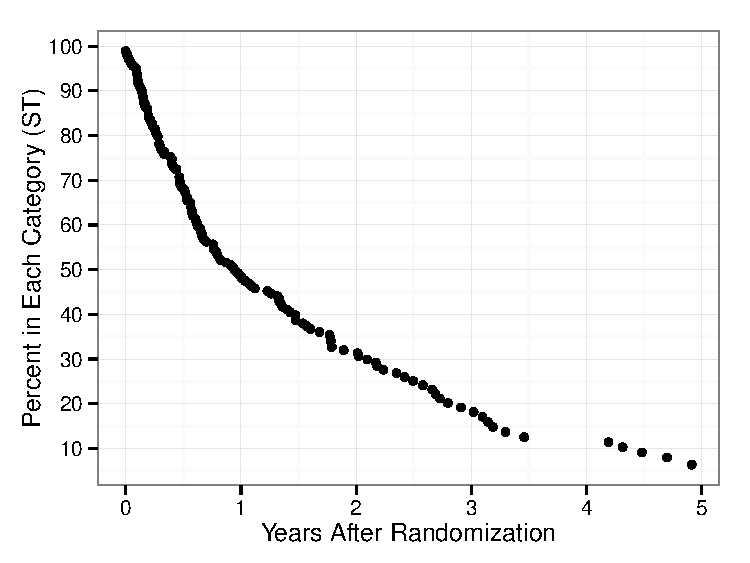
\includegraphics[width=\maxwidth]{figure/beamer-points} 

}

\caption[Point Plot]{Point Plot\label{F:points}}
\end{figure}


\end{knitrout}
Once we have added data to the \code{ggplot} object, we can display the figure as shown in Figure~\ref{F:points}. Until know the figure has been manipulated by sequentially adding function calls to the \code{ccf_plot} object. To display the figure you can either use the \code{show()} function, or simply use the object name at the command line.

Note that we have used the default \emph{shape}, \emph{size} and \emph{color} for this figure. These can be manipulated by adding arguments to the \code{geom_} functions, outside of the \code{aes()} function, as we will demonstrate in the following sections.

\subsection{ErrorBars}\label{S:errorbars}

Instead of using a single function to set points, lines and error bars, \pkg{ggplot2} uses individual function calls to control these elements. The \code{geom_errorbar} function takes the same arguments as the other \code{geom_} functions. However, since an errorbar is defined with upper and lower limits, we need to supply an \code{ymax} and \code{ymin} argument to the graphic aesthetic function. This code chunk plots both points, and error bars for the next two data series, the \code{sgdead1} variable with errorbars running from \code{stldead1} to \code{studead1} and \code{sgstrk1} variable with errorbars running from \code{stlstrk1} to \code{stustrk1}. As we see in Figure~\ref{F:errorBars}, both series were added in \code{color="blue"}, with different point shapes (\code{shape=1} and \code{shape=0}). We manipulated the error bar size with the \code{width} argument

\begin{knitrout}\footnotesize
\definecolor{shadecolor}{rgb}{0.969, 0.969, 0.969}\color{fgcolor}\begin{kframe}
\begin{alltt}
\hlcom{#     tuple set=green, symbol=circle, symbsize=1/2, linepe=0, linecl=0,}
\hlcom{#       ebarsize=3/4, ebar=1,}
\hlcom{#       x=iv_state, y=sgdead1, cll=stldead1, clu=studead1, color=blue, end;}
\hlstd{ccf_plot} \hlkwb{<-} \hlstd{ccf_plot} \hlopt{+}
  \hlkwd{geom_point}\hlstd{(}\hlkwc{data}\hlstd{=nonparametric,} \hlkwd{aes}\hlstd{(}\hlkwc{x}\hlstd{=iv_state,} \hlkwc{y}\hlstd{=sgdead1),}\hlkwc{color}\hlstd{=}\hlstr{"blue"}\hlstd{,}\hlkwc{shape}\hlstd{=}\hlnum{1}\hlstd{)} \hlopt{+}
  \hlkwd{geom_errorbar}\hlstd{(}\hlkwc{data}\hlstd{=nonparametric,} \hlkwd{aes}\hlstd{(}\hlkwc{x}\hlstd{=iv_state,} \hlkwc{ymin}\hlstd{=stldead1,} \hlkwc{ymax}\hlstd{=studead1),}
                \hlkwc{color}\hlstd{=}\hlstr{"blue"}\hlstd{,} \hlkwc{width}\hlstd{=}\hlnum{.1}\hlstd{)}

\hlcom{#      tuple set=green, symbol=square, symbsize=1/2, linepe=0, linecl=0,}
\hlcom{#       ebarsize=3/4, ebar=1,}
\hlcom{#       x=iv_state, y=sgstrk1, cll=stlstrk1, clu=stustrk1, color=blue, end;}
\hlstd{ccf_plot} \hlkwb{<-} \hlstd{ccf_plot} \hlopt{+}
  \hlkwd{geom_point}\hlstd{(}\hlkwc{data}\hlstd{=nonparametric,} \hlkwd{aes}\hlstd{(}\hlkwc{x}\hlstd{=iv_state,} \hlkwc{y}\hlstd{=sgstrk1),}\hlkwc{color}\hlstd{=}\hlstr{"blue"}\hlstd{,}\hlkwc{shape}\hlstd{=}\hlnum{0}\hlstd{)} \hlopt{+}
  \hlkwd{geom_errorbar}\hlstd{(}\hlkwc{data}\hlstd{=nonparametric,} \hlkwd{aes}\hlstd{(}\hlkwc{x}\hlstd{=iv_state,} \hlkwc{ymin}\hlstd{=stlstrk1,} \hlkwc{ymax}\hlstd{=stustrk1),}
                \hlkwc{color}\hlstd{=}\hlstr{"blue"}\hlstd{,} \hlkwc{width}\hlstd{=}\hlnum{.1}\hlstd{)}

\hlkwd{show}\hlstd{(ccf_plot)}
\end{alltt}


{\ttfamily\noindent\color{warningcolor}{Warning: Removed 7 rows containing missing values (geom\_point).\\Warning: Removed 117 rows containing missing values (geom\_point).}}\end{kframe}\begin{figure}[htpb]


{\centering 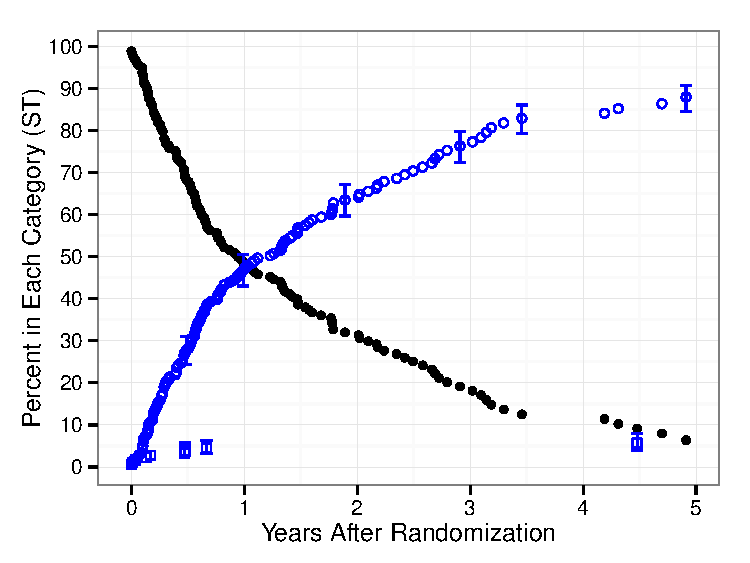
\includegraphics[width=\maxwidth]{figure/beamer-errorBars} 

}

\caption[Error Bar Plot]{Error Bar Plot\label{F:errorBars}}
\end{figure}


\end{knitrout}

Note that the \code{x} variable is the same for all three data series and the associated error bars. Also, since we do not want an error bar at every data point, a large number points have the upper and lower error bar variables set to \code{NA}. This is the same behavior as the \code{plot.sas} macro. \pkg{ggplot2} does print warnings when we attempt to plot a series with missing values. We typically suppress those warnings, but left them here for illustration purposes only.

\subsection{Lines}\label{S:lines}
Similar to points and error bars, the \code{geom_line} function is used to plot lines. We use the \code{linetype} argument to specify the line styles. We do have to generate a seperate \code{geom_line} function call for each limit of the confidence limit, since it is constructed of two lines (the upper and lower confidence limit). Alternatively, we can use the \code{geom_ribbon} to generate the confidence band using a shaded region and only a single call. The aesthetic argument for \code{geom_ribbon} takes a \code{ymax} and \code{ymin} argument just as the \code{geom_errorbar} function.
\begin{knitrout}\footnotesize
\definecolor{shadecolor}{rgb}{0.969, 0.969, 0.969}\color{fgcolor}\begin{kframe}
\begin{alltt}
\hlcom{# /**********PARAMETRIC : SOLID LINES AND CONFIDENCE INTERVALS**********/      }
\hlcom{# tuple set=all, x=years, y=noinit, cll=clinit, clu=cuinit,}
\hlcom{# width=0.5,color=black, end;}

\hlstd{ccf_plot} \hlkwb{<-} \hlstd{ccf_plot}\hlopt{+}
  \hlkwd{geom_line}\hlstd{(}\hlkwc{data}\hlstd{=parametric,} \hlkwd{aes}\hlstd{(}\hlkwc{x}\hlstd{=years,} \hlkwc{y}\hlstd{=noinit))}\hlopt{+}
  \hlkwd{geom_line}\hlstd{(}\hlkwc{data}\hlstd{=parametric,} \hlkwd{aes}\hlstd{(}\hlkwc{x}\hlstd{=years,} \hlkwc{y}\hlstd{=clinit),} \hlkwc{linetype}\hlstd{=}\hlstr{"dashed"}\hlstd{)}\hlopt{+}
  \hlkwd{geom_line}\hlstd{(}\hlkwc{data}\hlstd{=parametric,} \hlkwd{aes}\hlstd{(}\hlkwc{x}\hlstd{=years,} \hlkwc{y}\hlstd{=cuinit),} \hlkwc{linetype}\hlstd{=}\hlstr{"dashed"}\hlstd{)}
\hlcom{# }
\hlcom{# tuple set=all, x=years, y=nodeath, cll=cldeath, clu=cudeath,}
\hlcom{# width=0.5,color=blue, end;}
\hlstd{ccf_plot} \hlkwb{<-} \hlstd{ccf_plot}\hlopt{+}
  \hlkwd{geom_line}\hlstd{(}\hlkwc{data}\hlstd{=parametric,} \hlkwd{aes}\hlstd{(}\hlkwc{x}\hlstd{=years,} \hlkwc{y}\hlstd{=nodeath),} \hlkwc{color}\hlstd{=}\hlstr{"blue"}\hlstd{)}\hlopt{+}
  \hlkwd{geom_line}\hlstd{(}\hlkwc{data}\hlstd{=parametric,} \hlkwd{aes}\hlstd{(}\hlkwc{x}\hlstd{=years,} \hlkwc{y}\hlstd{=cldeath),} \hlkwc{linetype}\hlstd{=}\hlstr{"dashed"}\hlstd{,} \hlkwc{color}\hlstd{=}\hlstr{"blue"}\hlstd{)}\hlopt{+}
  \hlkwd{geom_line}\hlstd{(}\hlkwc{data}\hlstd{=parametric,} \hlkwd{aes}\hlstd{(}\hlkwc{x}\hlstd{=years,} \hlkwc{y}\hlstd{=cudeath),} \hlkwc{linetype}\hlstd{=}\hlstr{"dashed"}\hlstd{,} \hlkwc{color}\hlstd{=}\hlstr{"blue"}\hlstd{)}
\hlcom{# }
\hlcom{# tuple set=all, x=years, y=nostrk, cll=clstrk, clu=custrk,}
\hlcom{# linecl=2, width=0.5,color=blue, end;}
\hlstd{ccf_plot} \hlkwb{<-} \hlstd{ccf_plot}\hlopt{+}
  \hlkwd{geom_line}\hlstd{(}\hlkwc{data}\hlstd{=parametric,} \hlkwd{aes}\hlstd{(}\hlkwc{x}\hlstd{=years,} \hlkwc{y}\hlstd{=nostrk),} \hlkwc{color}\hlstd{=}\hlstr{"blue"}\hlstd{)}\hlopt{+}
  \hlkwd{geom_line}\hlstd{(}\hlkwc{data}\hlstd{=parametric,} \hlkwd{aes}\hlstd{(}\hlkwc{x}\hlstd{=years,} \hlkwc{y}\hlstd{=clstrk),} \hlkwc{linetype}\hlstd{=}\hlstr{"dashed"}\hlstd{,} \hlkwc{color}\hlstd{=}\hlstr{"blue"}\hlstd{)}\hlopt{+}
  \hlkwd{geom_line}\hlstd{(}\hlkwc{data}\hlstd{=parametric,} \hlkwd{aes}\hlstd{(}\hlkwc{x}\hlstd{=years,} \hlkwc{y}\hlstd{=custrk),} \hlkwc{linetype}\hlstd{=}\hlstr{"dashed"}\hlstd{,} \hlkwc{color}\hlstd{=}\hlstr{"blue"}\hlstd{)}

\hlkwd{show}\hlstd{(ccf_plot)}
\end{alltt}
\end{kframe}\begin{figure}[htpb]


{\centering 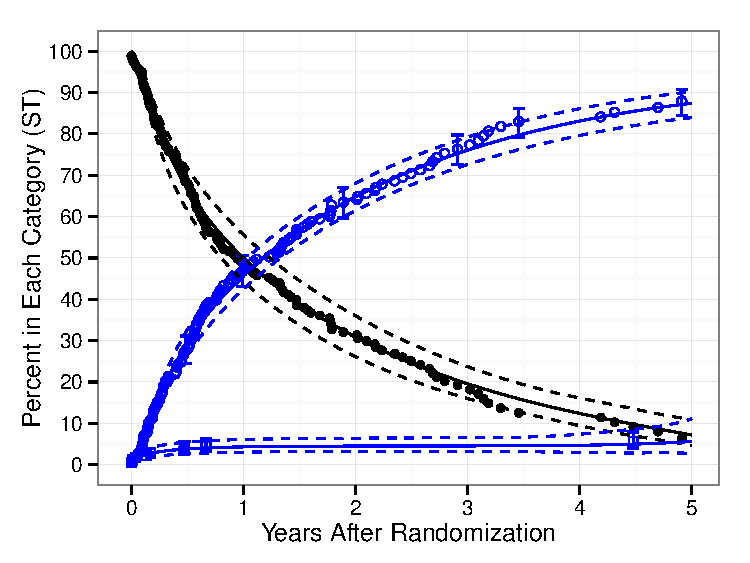
\includegraphics[width=\maxwidth]{figure/beamer-lines} 

}

\caption[Line Plot with confidence bands]{Line Plot with confidence bands\label{F:lines}}
\end{figure}


\end{knitrout}

This time, we used the \code{parametric} data set in the \code{data} argument, as we want to use a different set of points for generating these lines. 

\subsection{Linetypes}\label{S:linetypes}
The \code{linetype} argument takes a named string as a value, to set the different line styles. The set of styles is shown in Figure~\ref{F:linetypes}. 
\begin{knitrout}\footnotesize
\definecolor{shadecolor}{rgb}{0.969, 0.969, 0.969}\color{fgcolor}\begin{figure}[htpb]


{\centering 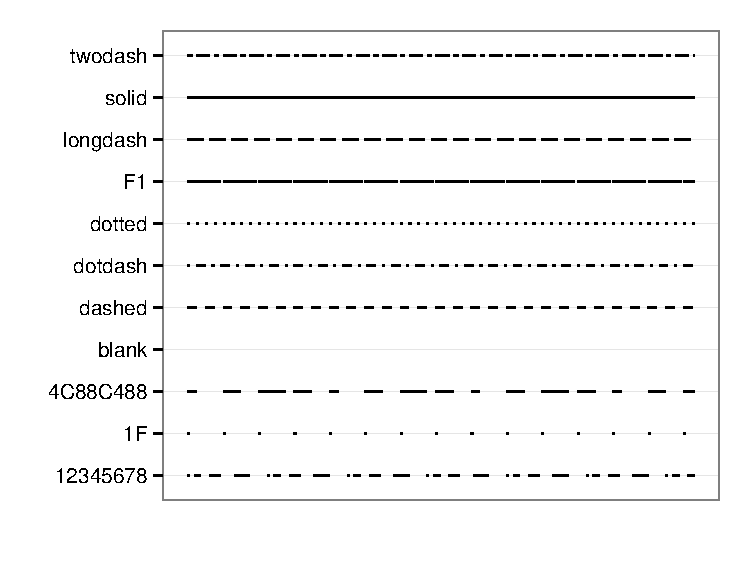
\includegraphics[width=\maxwidth]{figure/beamer-linetypes} 

}

\caption[ggplot2 linetype table]{ggplot2 linetype table\label{F:linetypes}}
\end{figure}


\end{knitrout}

\subsection{Shapes}\label{S:shapes}
The \code{shape} argument takes numeric arguments. Though not user freindly, it is at least consistent. Figure~\ref{F:shapes} shows the catalog of shapes with corresponding numeric argument constructed using the ones place along the x-axis, and tens along the y-axis. So the filled dot, default point shape shown in black in Figure~\ref{F:lines} is shape 20.

\begin{knitrout}\footnotesize
\definecolor{shadecolor}{rgb}{0.969, 0.969, 0.969}\color{fgcolor}\begin{figure}[htpb]


{\centering 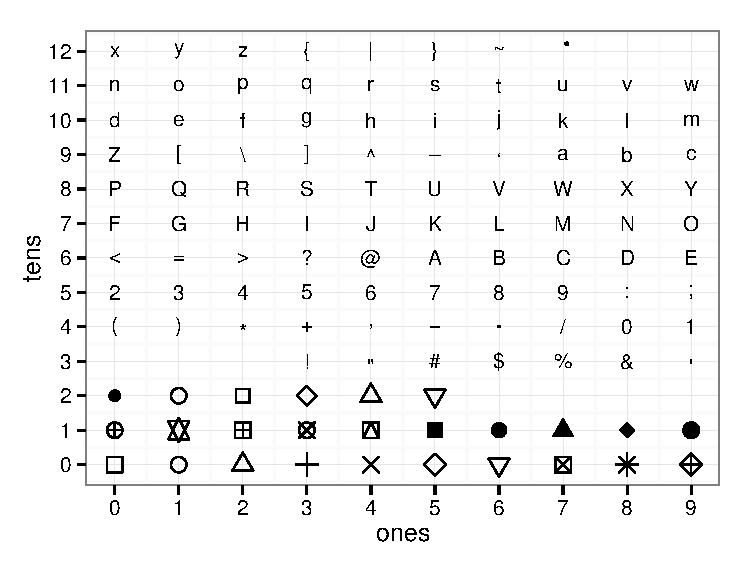
\includegraphics[width=\maxwidth]{figure/beamer-shapes} 

}

\caption[ggplot2 shape table]{ggplot2 shape table\label{F:shapes}}
\end{figure}


\end{knitrout}

\subsection{Colors}\label{S:colors}
You can specify colors in \proglang{R} by numeric index, name (as we have done), hexadecimal, or RGB specification. For example \code{col=1} and \code{col="white"}  are equivalent. The chart in Figure~\ref{F:colorChart} was produced with code developed by~\cite{Glynn:2005}. See his \proglang{R}  Color Chart website for all the details you would ever need about using colors in R.

\begin{knitrout}\footnotesize
\definecolor{shadecolor}{rgb}{0.969, 0.969, 0.969}\color{fgcolor}\begin{figure}[htpb]


{\centering 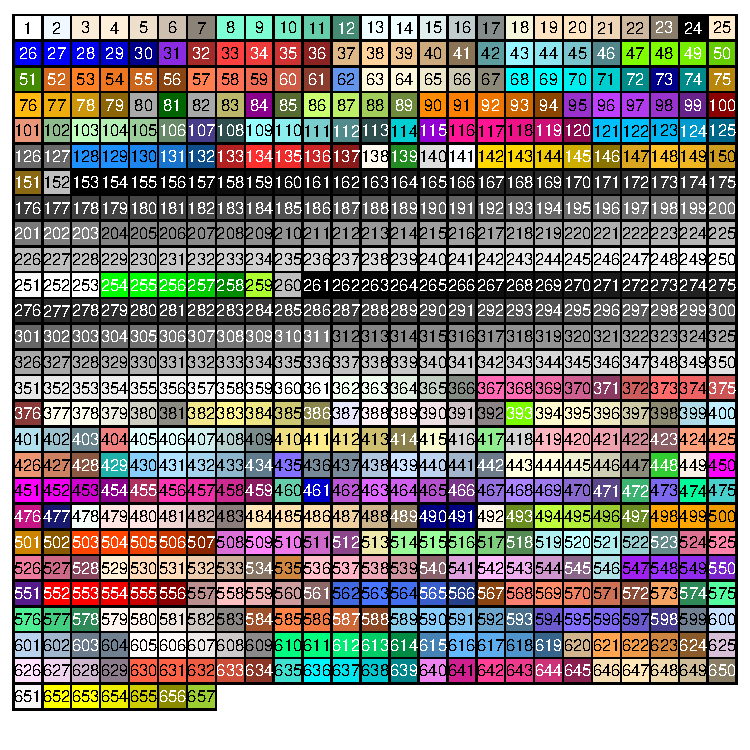
\includegraphics[width=\maxwidth]{figure/beamer-colorChart} 

}

\caption[R colors]{R colors\label{F:colorChart}}
\end{figure}


\end{knitrout}

Color theory encompasses a multitude of definitions, concepts and design applications - enough to fill several encyclopedias. However, there are three basic categories of color theory that are logical and useful : The color wheel, color harmony, and the context of how colors are used. ColorBrewer~\citep{Brewer:2003} is an online tool~(\url{http://colorbrewer2.org/}) designed to help people select good color schemes for maps and other graphics. We encourage the use of ColorBrewer as a good, safe introduction to selecting colors based on theoretically good practices. 

The \pkg{RColorBrewer} package~citep{Neuwirth:2011} simplifies the selection of ColorBrewer colors into \proglang{R}. We have used \pkg{RColorBrewer} to get a list of colors, and assign colors manually to specific variable values using the \pkg{ggplot2} \code{aes()} mechanism. The ColorBrewer palletes have also been built into the \pkg{ggplot2} \code{scale_} functions in the \code{scale_color_brewer} function. We have made extensive use of the \code{palette="Set1"} color palette in figures we have generated. There are also a series of other \code{scale_color_} functions in \pkg{ggplot2} to aid the user in selecting good color schemes for many different settings.

\subsection{Global Commands}\label{S:globals}

\begin{knitrout}\footnotesize
\definecolor{shadecolor}{rgb}{0.969, 0.969, 0.969}\color{fgcolor}\begin{kframe}
\begin{alltt}
\hlcom{# Special commands to force origin to 0,0}
\hlstd{ccf_plot} \hlkwb{<-} \hlstd{ccf_plot} \hlopt{+}
  \hlkwd{coord_cartesian}\hlstd{(}\hlkwc{xlim}\hlstd{=}\hlkwd{c}\hlstd{(}\hlnum{0}\hlstd{,}\hlnum{5.2}\hlstd{),} \hlkwc{ylim}\hlstd{=}\hlkwd{c}\hlstd{(}\hlnum{0}\hlstd{,}\hlnum{101}\hlstd{))}

\hlkwd{show}\hlstd{(ccf_plot)}
\end{alltt}
\end{kframe}\begin{figure}[htpb]


{\centering 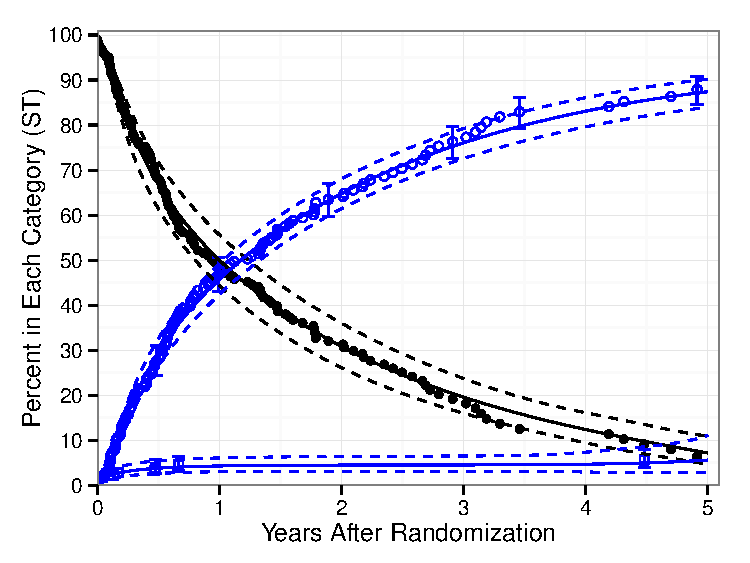
\includegraphics[width=\maxwidth]{figure/beamer-global_} 

}

\caption[Adjusting the viewport]{Adjusting the viewport\label{F:global,}}
\end{figure}


\end{knitrout}

% #   expand_limits(x = 0, y = 0) +
% #   scale_x_continuous(expand = c(-0.1, 0.1)) + 
% #   scale_y_continuous(expand = c(-1, 0.1))

% -----------------------------------------------------
\section{PowerPoint Figures}\label{S:powerPointFigures}
% -----------------------------------------------------

As a second example, we recreate a figure that was created for PowerPoint with the \code{plot.sas} macro. In most cases, we do not include points when generating presentation figures, so this figure was generated with only \code{geom_line} function calls. We also show how the figure can be created in a single set of function calls.

\begin{knitrout}\footnotesize
\definecolor{shadecolor}{rgb}{0.969, 0.969, 0.969}\color{fgcolor}\begin{kframe}
\begin{alltt}
\hlcom{# %plot(goptions gsfmode=replace, device=cgmmppa, ftext=hwcgm001, end;}
\hlcom{# axisx order=(0 to 5 by 1), minor=none, value=(height=2.4), end;}
\hlcom{# axisy order=(0 to 100 by 20), minor=none, value=(height=2.4), }
\hlcom{# value=(height=2.4 j=r ' ' '20' '40' '60' '80' '100'), end;}
\hlcom{# tuple set=all, x=years, y=noinit, width=3, color=gray, end;}
\hlcom{# tuple set=all, x=years, y=nostrk, width=3, color=red, end;}
\hlcom{# tuple set=all, x=years, y=nodeath, width=3, color=blue, end;}
\hlcom{# );}
\hlstd{ccf_pptPlot} \hlkwb{<-} \hlkwd{ggplot}\hlstd{()}\hlopt{+}
  \hlkwd{scale_x_continuous}\hlstd{(}\hlkwc{breaks}\hlstd{=}\hlkwd{seq}\hlstd{(}\hlnum{0}\hlstd{,}\hlnum{5}\hlstd{,}\hlnum{1}\hlstd{))}\hlopt{+}
  \hlkwd{scale_y_continuous}\hlstd{(}\hlkwc{breaks}\hlstd{=}\hlkwd{seq}\hlstd{(}\hlnum{0}\hlstd{,}\hlnum{100}\hlstd{,}\hlnum{20}\hlstd{))}\hlopt{+}
  \hlkwd{geom_line}\hlstd{(}\hlkwc{data}\hlstd{=parametric,} \hlkwd{aes}\hlstd{(}\hlkwc{x}\hlstd{=years,} \hlkwc{y}\hlstd{=noinit),} \hlkwc{color}\hlstd{=}\hlstr{"grey"}\hlstd{,} \hlkwc{size}\hlstd{=}\hlnum{1.5}\hlstd{)}\hlopt{+}
  \hlkwd{geom_line}\hlstd{(}\hlkwc{data}\hlstd{=parametric,} \hlkwd{aes}\hlstd{(}\hlkwc{x}\hlstd{=years,} \hlkwc{y}\hlstd{=nostrk),} \hlkwc{color}\hlstd{=}\hlstr{"red"}\hlstd{,} \hlkwc{size}\hlstd{=}\hlnum{1.5}\hlstd{)}\hlopt{+}
  \hlkwd{geom_line}\hlstd{(}\hlkwc{data}\hlstd{=parametric,} \hlkwd{aes}\hlstd{(}\hlkwc{x}\hlstd{=years,} \hlkwc{y}\hlstd{=nodeath),} \hlkwc{color}\hlstd{=}\hlstr{"blue"}\hlstd{,} \hlkwc{size}\hlstd{=}\hlnum{1.5}\hlstd{)}

\hlkwd{show}\hlstd{(ccf_pptPlot)}
\end{alltt}
\end{kframe}\begin{figure}[htpb]


{\centering 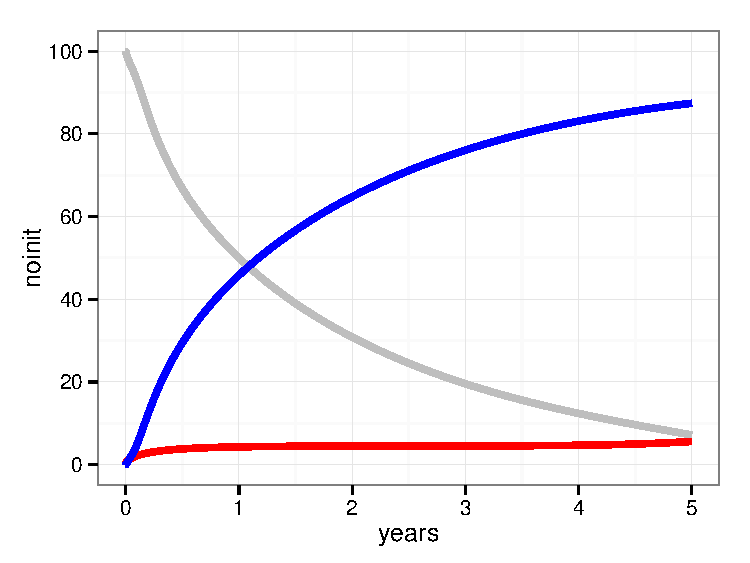
\includegraphics[width=\maxwidth]{figure/beamer-powerpoint} 

}

\caption[PowerPoint Figures]{PowerPoint Figures\label{F:powerpoint}}
\end{figure}


\end{knitrout}


% -----------------------------------------------------
\section[Themes for publications]{\pkg{ggplot2} themes for publication}\label{S:themes}
% -----------------------------------------------------

\subsection{Theme for Manuscripts}


\begin{knitrout}\footnotesize
\definecolor{shadecolor}{rgb}{0.969, 0.969, 0.969}\color{fgcolor}\begin{kframe}
\begin{alltt}
\hlcom{# Set the theme for manuscripts,}
\hlkwd{theme_set}\hlstd{(}\hlkwd{theme_man}\hlstd{())}

\hlcom{# show the figure.}
\hlstd{ccf_plot}

\hlcom{# Reset the theme to the resonable default used previously.}
\hlkwd{theme_set}\hlstd{(}\hlkwd{theme_bw}\hlstd{())}
\end{alltt}
\end{kframe}\begin{figure}[htpb]


{\centering 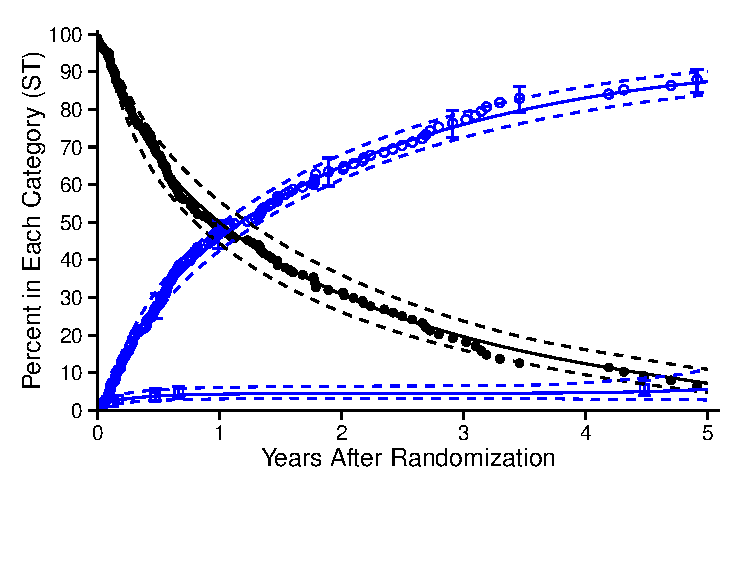
\includegraphics[width=\maxwidth]{figure/beamer-manuscriptTheme} 

}

\caption[Theme for Manuscripts]{Theme for Manuscripts\label{F:manuscriptTheme}}
\end{figure}


\end{knitrout}


\subsection{Theme for Presentations}\label{S:themesPPT}

\begin{knitrout}\footnotesize
\definecolor{shadecolor}{rgb}{0.969, 0.969, 0.969}\color{fgcolor}\begin{kframe}
\begin{alltt}
\hlcom{# Update the PowerPoint Figure to include the PPT Theme, and remove axis labels.}
\hlcom{# Axis labels will be added manually in powerpoint.}
\hlstd{ccf_pptPlot} \hlkwb{<-} \hlstd{ccf_pptPlot}\hlopt{+}
  \hlkwd{labs}\hlstd{(}\hlkwc{x}\hlstd{=}\hlstr{""}\hlstd{,}\hlkwc{y}\hlstd{=}\hlstr{""}\hlstd{)}\hlopt{+}
  \hlkwd{theme_ppt}\hlstd{()}

\hlcom{# Show the figure... the theme statement is used so the axis tick marks and values}
\hlcom{# are visible in this document.}
\hlstd{ccf_pptPlot} \hlopt{+}
  \hlkwd{theme}\hlstd{(}\hlkwc{plot.background} \hlstd{=} \hlkwd{element_rect}\hlstd{(}\hlkwc{fill}\hlstd{=}\hlstr{'blue'}\hlstd{,} \hlkwc{colour}\hlstd{=}\hlstr{'blue'}\hlstd{))}
\end{alltt}
\end{kframe}\begin{figure}[htpb]


{\centering 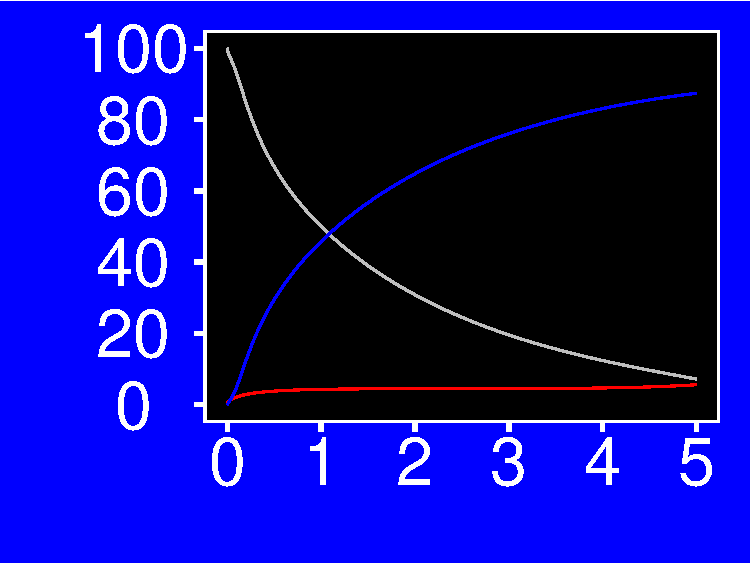
\includegraphics[width=\maxwidth]{figure/beamer-powerpointTheme} 

}

\caption[Theme for Presentations]{Theme for Presentations\label{F:powerpointTheme}}
\end{figure}


\end{knitrout}

% -----------------------------------------------------
\section{Saving Publication graphics}\label{S:saving}
% -----------------------------------------------------

\subsection{Manuscript graphics}



\begin{knitrout}\footnotesize
\definecolor{shadecolor}{rgb}{0.969, 0.969, 0.969}\color{fgcolor}\begin{kframe}
\begin{alltt}
\hlkwd{library}\hlstd{(gridExtra)}

\hlstd{ccf_savePlot} \hlkwb{<-} \hlkwd{arrangeGrob}\hlstd{(ccf_plot,}
                            \hlkwc{sub} \hlstd{=} \hlkwd{textGrob}\hlstd{(}\hlkwd{getwd}\hlstd{(),}
                                           \hlkwc{x} \hlstd{=} \hlnum{0}\hlstd{,} \hlkwc{hjust} \hlstd{=} \hlopt{-}\hlnum{.01}\hlstd{,} \hlkwc{vjust}\hlstd{=}\hlnum{1}\hlstd{,}
                                           \hlkwc{gp} \hlstd{=} \hlkwd{gpar}\hlstd{(}\hlkwc{fontface} \hlstd{=} \hlstr{"italic"}\hlstd{,} \hlkwc{fontsize} \hlstd{=} \hlnum{10}\hlstd{)))}
\hlstd{ccf_savePlot}
\end{alltt}
\end{kframe}

{\centering 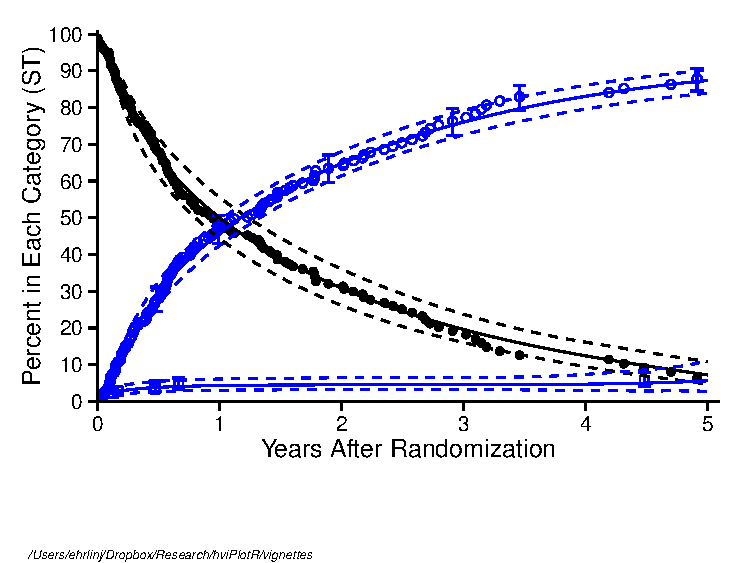
\includegraphics[width=\maxwidth]{figure/beamer-manuscriptFootnote} 

}



\end{knitrout}


ggsav
\subsection{PowerPoint graphics}
We use the \pkg{ReporteRs} package~\citep{Gohel:2014} to insert vector based figures from \proglang{R} into PowerPoint documents. The latest version of the \pkg{ReporteRs} package is available from \url{http://davidgohel.github.io/ReporteRs/}. We install this package as we installed the \pkg{hviPlotR} package.
\begin{knitrout}\footnotesize
\definecolor{shadecolor}{rgb}{0.969, 0.969, 0.969}\color{fgcolor}\begin{kframe}
\begin{alltt}
\hlcom{# Install the latest ReporteRs package.}
\hlcom{#}
\hlcom{# The devtools package is installed on all our }
\hlcom{# jjnb-gen servers as well as other R instances.}
\hlkwd{library}\hlstd{(devtools)}

\hlcom{# To get the latest version.}
\hlkwd{install_github}\hlstd{(}\hlstr{"davidgohel/ReporteRs"}\hlstd{)}
\end{alltt}
\end{kframe}
\end{knitrout}

Basically, the package works by opening a saved PowerPoint Presentation, and inserting new slides containing graphs or tables into the document. The resulting document is then saved to a new presentation. We then pass this presentation to our collaborators, who then copy and paste the \pkg{ggplot2} slides into their own presentations. 

The \pkg{ggplot2} graphics that are inserted into the presentation are converted into an editable vector based format. When the document is edited in PowerPoint, graphical components like points, lines, text can be easily modified to match the presenters style.

The following code block is an \proglang{R} recipe for saving the \code{ccf_pptPlot} created in Section~\ref{S:themesPPT}. 
\begin{knitrout}\footnotesize
\definecolor{shadecolor}{rgb}{0.969, 0.969, 0.969}\color{fgcolor}\begin{kframe}
\begin{alltt}
\hlkwd{library}\hlstd{(ReporteRs)}
\hlcom{# Create a powerPoint document using ../inst/RDPresentation.pptx }
\hlcom{# as a template document.}
\hlstd{doc} \hlkwb{=} \hlkwd{pptx}\hlstd{(}\hlkwc{template}\hlstd{=}\hlkwd{paste}\hlstd{(}\hlstr{"../inst/RDPresentation.pptx"}\hlstd{,} \hlkwc{sep}\hlstd{=}\hlstr{""}\hlstd{))}

\hlcom{# Here we define powerpoint document filename to write}
\hlcom{# the presentation. This will be overwritten}
\hlstd{pptx.file} \hlkwb{=} \hlkwd{paste}\hlstd{(}\hlstr{"RDExample.pptx"}\hlstd{,} \hlkwc{sep}\hlstd{=}\hlstr{""}\hlstd{)}

\hlcom{##--------}
\hlcom{# For each graph, addSlide. The graphs require the }
\hlcom{# “Title and Content” template.}
\hlstd{doc} \hlkwb{=} \hlkwd{addSlide}\hlstd{( doc,} \hlstr{"Title and Content"} \hlstd{)}

\hlcom{# Place a title}
\hlstd{doc} \hlkwb{=} \hlkwd{addTitle}\hlstd{( doc,} \hlstr{"Treatment Difference"} \hlstd{)}

\hlcom{# Now add the graph into the powerPoint doc }
\hlstd{doc} \hlkwb{=} \hlkwd{addPlot}\hlstd{(} \hlkwc{doc}\hlstd{=doc,} \hlkwc{fun}\hlstd{=print,}
               \hlkwc{x}\hlstd{=ccf_pptPlot}\hlopt{+}\hlkwd{theme_ppt}\hlstd{() ,}
               \hlkwc{editable} \hlstd{=} \hlnum{TRUE}\hlstd{,}
               \hlkwc{offx}\hlstd{=}\hlnum{.75}\hlstd{,} \hlkwc{offy}\hlstd{=}\hlnum{1.1}\hlstd{,} \hlkwc{width}\hlstd{=}\hlnum{8}\hlstd{,} \hlkwc{height}\hlstd{=}\hlnum{6}\hlstd{)}
\hlcom{##--------}
\hlcom{## IF you want to add more, just repeat between the ##-------- comments}
\hlcom{##--------}

\hlcom{# write the output powerpoint doc. }
\hlcom{# This will not overwrite an open document, since open PPT files are locked.}
\hlkwd{writeDoc}\hlstd{( doc, pptx.file )}
\end{alltt}
\end{kframe}
\end{knitrout}

The only modification possibly require for this recipe may be moving the insertion point (\code{offx} and \code{offy} arguments) and/or size (\code{width} and \code{height}) of the figure in the \code{addPlot()} function call.

% -----------------------------------------------------
\section{Generating other figure types}\label{S:alternateFigures}
% -----------------------------------------------------

\subsection{Bar Charts}

\subsection{Histograms}

\subsection{Additional Figure Types}


% -----------------------------------------------------
\section{Graphics rules to live by}\label{S:rules}
% -----------------------------------------------------

% =======================================
\section{Conclusions} \label{S:concl}
% =======================================
In this article, we present some functions in the \pkg{hviPlotR} package for \proglang{R} 

% =======================================
% \section{Literatur} \label{sec: references}
% =======================================
%\nocite{*}

\bibliography{hviPlotR}



\end{document}
